\Chapter{PERFORMANCE SIGNATURE APPROACH}\label{sec:Approach}

This chapter presents the method we introduce to determine the model that is closest to the ground truth for a given data set.  We refer to this method as ``Performance Signature'' approach, or ``Signature'' approach for short. 

The basic principles of the method is to define a vector space of model performances, namely the models described in chapter \ref{sec:RevLitt}.  Then, synthetic data is created with each model, and each model's performances are measured over each of the synthetic data set.  These measures represent a point in that space. The synthetic data point associated with that point represents the ground thruth prototype, or the centroid for classification.  Given a new data set, we use a nearest neighbor approach with a correlation distance to identify the closest ground truth model.

Let us rephrase the method in more general terms and consider a set of models, $\mathcal{M}$, and a vector~$\mathbf{p}$ of length~$|\mathcal{M}|$ that contains the performance of each model over a given data set.  This vector represents a point in the performance space.  For each model $M \in \mathcal{M}$, we determine a point in the performance space that corresponds to synthetic data generated with model~$M$.  Then, for a given data set, we find the nearest synthetic data set point, using correlation as a distance, and consider the model behind it to be the ground thruth.

\note{Let's ask Peng to see if this more formal formulation is correct and if it can be improved.}

The rest of the chapter goes into more details about the method.

% \section{Synthetic data}
% This approach relies on synthetic data. A unique advantage of synthetic data is that the model parameters can be predefined. Once the simulated data is generated with predefined parameters, a model can be trained over the generated data and a comparison with the original, known parameter values becomes possible. This may be the strongest benefit of synthetic data in assessing model fit since the hypothesis of this research relies on comparison the performance vector of real vs. synthetic data.

% Generating data is a complex task because sometimes it requires many parameters. Some parameters are dependent on the model which is the base of generation. Regardless of the type of the base model, some others are always essential which are data specific parameters such as sample size and score variance. 

% Given that our objective is to determine the ground thruth of a given data set, we will borrow data specific parameters from this data set to generate the synthetic data.  Further details are given in chapter~\ref{sec:Syn}. 


\section{Model fit in a vector space framework}

% This approach is based on the assumption that the predictive performance of a given model will vary as a function of the data set's groud truth model, and that the performance vector between different data sets will be stable.

Let us explain the general idea with the performance data in table~\ref{tab:vectorspace}, where the predictive accuracy of the 6~models reviewed in chapter~\ref{sec:RevLitt} is reported against 6~synthetic data sets generated with the same models.  A seventh ``model'' named \textit{expected} (section~\ref{sec:basel-expect-pred}) and a seventh data set named \textit{random} (random results that constrained to reflect the target data set parameters such as item and student success rate distribution) are added for comparison purpose.  

\newcolumntype{d}[1]{D{.}{.}{#1}} % not used

\begin{table}[ht]
\caption{Vector space of accuracy performances}\label{tab:vectorspace}
\centering
\begin{tabular}{lccccccc}
  \toprule
  \multicolumn{1}{c}{\multirow{2}{*}{\textbf{Model}}} & \multicolumn{7}{c}{\textbf{Synthetic data set }\tablefootnote{Note that the Synthetic datasets are generated based on different models. Namely, IRT means that the ground truth of the generated dataset assumed to be IRT model}} \\
  \cline{2-8}
  & \multicolumn{1}{c}{{\textit{Random}}} & \multicolumn{1}{c}{{POKS}} & \multicolumn{1}{c}{{IRT}} & \multicolumn{1}{c}{{DINA}} & \multicolumn{1}{c}{{DINO}} & \multicolumn{1}{c}{{Linear .Conj}} & \multicolumn{1}{c}{{Linear .Comp}} \\ 
  \hline
  \textit{Expected} & \textbf{0.75} & 0.91 & 0.90 & 0.72 & 0.72 & 0.78 & 0.93 \\ 
  POKS & 0.75 & \textbf{0.94} & 0.94 & 0.81 & 0.81 & 0.90 & 0.94 \\ 
  IRT & 0.75 & 0.91 & \textbf{0.95} & 0.73 & 0.73 & 0.79 & 0.89 \\ 
  DINA & 0.75 & 0.77 & 0.81 & \textbf{1.00} & 0.65 & \textbf{0.98} & 0.89 \\ 
  DINO & 0.75 & 0.63 & 0.56 & 0.66 & \textbf{1.00} & 0.68 & 0.91 \\ 
  NMF.Conj & 0.75& 0.59 & 0.53 & 0.95 & 0.65 & 0.97 & 0.58 \\ 
  NMF.Comp & 0.75 & 0.76 & 0.79 & 0.59 & 0.93 & 0.70 & \textbf{0.98} \\ 
  \bottomrule
\end{tabular}
\end{table}


As we can expect, the diagonal (in bold face, except for one), corresponding to the match between the underlying synthetic model and the model performance) generally displays the best performance since it corresponds to the alignment of the model and the ground truth behind the data.  This confirms the intuition behind the usual strategy of assuming the best performer is the model behind the ground truth.  However, this is not always the case. In this particular example, the DINA model show a better performance over the Linear Conj.\ data set, whereas this data set's corresponding model is the NMF Conj. 



The principle of the proposed approach is to use the whole column of performance as a vector to determine the closest model to the ground truth.  In that respect, if columns are considered as vectors in the space of dimensions created by model performances, we can use a similarity measure to determine the closest ground truth (or a distance measure if we consider the columns as a point in space).

The advantage of this approach is that it does not rely on a single performance value to determine the goodness of fit, but instead on a set of performances over different models.  The hypothesis is that this set of performances provides a more reliable measure of the goodness of fit of a set of models.  In turn, we assume that this measure is more likely to indicate which model will perform better in general, as opposed to which models performs the best in the case of the single data set at hand.  \note{This is where we could refer to an explicit hypothesis.}

The approach can be considered as a means to avoid a kind of local minimum, considering the best performer as a good indicator of the ground truth, but not a perfect one. Indeed, table~\ref{tab:vectorspace} suggests that aligning the model with the ground truth does yield the best performance except for one case, but we will show more examples later that there are exeptions and that the proposed approach is better able to avoid these exceptions that would lead to a wrong conclusion if we were to rely on the best performer approach.


\section{Research questions}

Let us get back to the research questions and design experiments for them, This section represents the framework of each designed experiment, later in chapter \ref{sec:SIGNATURE} the results of these experiment with more details will be given. To make it straightforward we break the contribution into four experiments:

\begin{enumerate}
\item What is the performance vector of student skills assessment models over real and over synthetic data created using the same models?
\begin{itemize}
\item Predictive performance: In a first experiment, we focus on showing the performance of all models described in chapter \ref{sec:RevLitt} over synthetic and real data sets.  It provides an overview of the predictive performance of each model across the different synthetic and real datasets. The output of this experiment is the predictive performance or the ``signature'' of the dataset.
\end{itemize}
\item Is the performance vector unique to each synthetic data type (data from the same ground truth model)?
\begin{itemize}
\item Sensitivity of the signature over different data specific parameters: This section tests the uniqueness of the signature over different data generation parameters.
\end{itemize}
%performance comparison
\item Can the performance vector be used to define a method to reliably identify the ground truth behind the synthetic data?
\begin{itemize}
\item Assessing the goodness of fit of a dataset: This part proposes a framework for model selection as well as a measure that represents the goodness of fit by comparing the predictive performance vector of the synthetic and real data.
\end{itemize}
\item How does the method compare with the standard practice of using the model with the best performance?  In particular, does the ground truth model identified better generalize over a space of parameter values?
\begin{itemize}
\item Generality of the proposed approach under different assumptions about the data: In a last experiment, we move focus to the central problem of this thesis: classifying data sets in the performance vector space.  To validate the approach, we need to rely on synthetic data for which we know the underlying ground truth model.  A matrix is created with data sets generated from the different models, and each model performance is measured through a cross validation process.  This matrix allows us to classify a data set of unknown ground truth according to a nearest neighbor approach. In fact, this experiment tests if the proposed approach remains reliable on different conditions of parameters and also measuring the accuracy of its performance to predict a ground truth in comparison with other approaches for different data parameter assumptions.
\end{itemize}
\end{enumerate}


\subsection{Predictive performance}

The performance of each model is assessed on the basis of 10-folds cross-validation.  The training set is used to estimate model parameters that are later used in for the test set. For each test set, a model is fed with a set of item outcomes of a student, called the observed set, and the remaining items are the predicted, or inferred ones. The breakdown of the data for cross-validation is illustrated in figure~\ref{figMethod}. We fixed the number of observed items for each run on each data set. The minimum number of observed items is 9 and the maximum number is one item less than total number of items. 

\begin{figure}[h]
\centering
{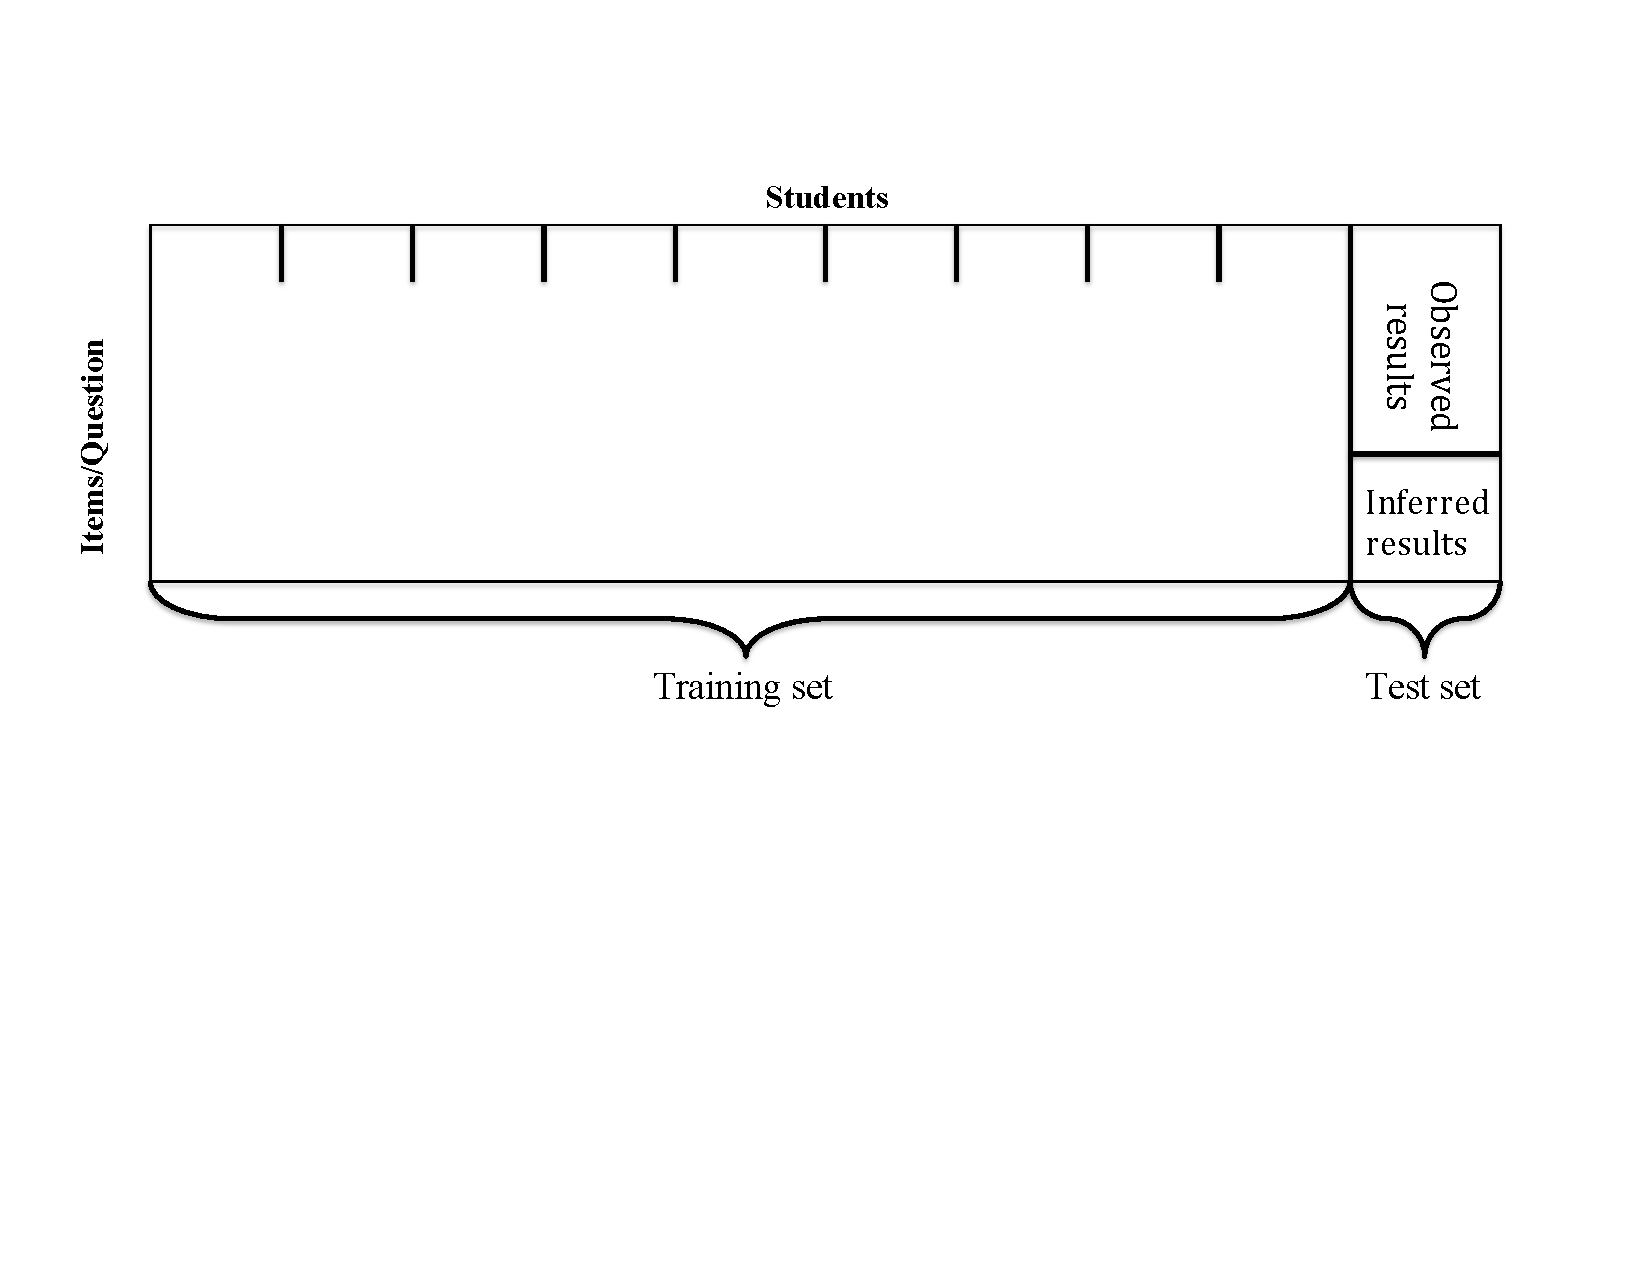
\includegraphics[trim=1cm 9cm 2.4cm 2.4cm,clip=true,width=.7\textwidth]{images/Methodology.pdf}}
\caption{Data breakdown of cross validation process}
\label{figMethod}
\end{figure}

For each dataset there exists a training set that contains 9 folds and a test set which represents a single fold. A list of required parameters are presented in table~\ref{fig:param}. Samples are assigned randomly to each fold and this setting is the same across all predictive models for each run. Since all items are presented in the training set, then we can estimate the parameters that are related to items to be used in the test set. 

For other parameters that are related to students we need to divide the test set into an observed and inferred set. From the observed set we can get to the parameters that are related to students. A list of required parameters for assessing the model performance in table~\ref{fig:param-Predictive-Performance} \footnote{Details of all parameters are given in chapter \ref{sec:Syn}}.

\newcommand{\tabitem}{~~\llap{\textbullet}~~}
\newcommand\VRule[1][\arrayrulewidth]{\vrule width #1}

\begin{table}[h]
  \centering

\begin{tabular}{c|c|l!{\VRule[1.5pt]}l|l!{\VRule[1.5pt]}l|}
\multicolumn{3}{c}{}&\multicolumn{3}{c}{Parameters estimated from}\tabularnewline
\cline{4-6}
\multicolumn{3}{c!{\VRule[1.5pt]}}{Skills Model}&\multicolumn{2}{c!{\VRule[1.5pt]}}{Training set}&Observed items\tabularnewline
\cmidrule[1.5pt]{2-6}
&&NMF Conj. & & &  \tabularnewline
\cline{3-3}
&&NMF Add.&&& \tabularnewline
\cline{3-4}
&&DINA& \tabitem Slip & &\tabularnewline
\cline{3-3} 
&\multirow{-4}{*}{\begin{sideways} \scriptsize Multiple\end{sideways}}&DINO& \tabitem Guess&\multirow{-4}{*}{ \tabitem  Q-matrix }&\multirow{-4}{*}{  \parbox[t]{3cm}{ \tabitem Students skills  \\ mastery matrix}} \tabularnewline
\cmidrule[1.5pt]{2-6}
&&&\multicolumn{2}{l!{\VRule[1.5pt]}}{\tabitem Item difficulty  } &  \tabularnewline
&&\multirow{-2}{*}{ IRT}&\multicolumn{2}{l!{\VRule[1.5pt]}}{\tabitem Item discrimination}  &\multirow{-2}{*}{\tabitem Student Ability} \tabularnewline
\cline{3-6}
&\multirow{-3}{*}{\begin{sideways} \scriptsize Single \end{sideways}}&Expected&\multicolumn{2}{l!{\VRule[1.5pt]}}{\tabitem Item Odds}  &\tabitem Student Odds \tabularnewline
\cmidrule[1.5pt]{2-6}
&&&\multicolumn{2}{l!{\VRule[1.5pt]}}{\tabitem Initial Odds } & \tabularnewline
&&&\multicolumn{2}{l!{\VRule[1.5pt]}}{ \tabitem Odds ratio } & \tabularnewline
\multirow{-9}{*}{\begin{sideways} \scriptsize Contributed skills \end{sideways}}&\multirow{-3}{*}{\begin{sideways} \scriptsize Zero\end{sideways}}&\multirow{-3}{*}{ POKS }&\multicolumn{2}{l!{\VRule[1.5pt]}}{\tabitem Partial order structure}&\multirow{-3}{*}{ }\tabularnewline
\cmidrule[1.5pt]{2-6}
\end{tabular}
  \caption{Parameters of the predictive performance framework}
  \label{fig:param-Predictive-Performance}
\end{table}

Once all the required parameters are presented we can make a prediction for the inferred cells of the result matrix. Note that the selected observed and inferred items are the same across all the models for each run to make a better comparison for their prediction. A probability of mastery is obtained and rounded, resulting in a 0/1 error loss function.  We report the mean accuracy as the performance measure later in chapter \ref{sec:SIGNATURE}.  The R package \texttt{ltm} is used for parameter and skills estimation for IRT model and the R package \texttt{CDM} and \texttt{NMF} for Deterministic Input Noisy and NMF models. 

\note{This is a description of experiments whose results are presented one chapter later.  Not ideal, but I understand it is also necessary to introduce the data generation chapter.  We may leave it as is, but I add this note for the moment}

\subsection{Sensitivity of the Model performance over data generation parameters}
\label{Sensitive}

%One interesting finding of the previous experiment on synthetic dataset was that the best performer model was the ground truth for the given set of parameters. 
In this experiment we want to examine the effect of data generation parameters on the stability of the model performance vector in the performance space. In this section we run the same experiment but with different data generation parameters such as average success rate, sample size, number of latent skills, number of items, student and item score variance. This research can answer the question whether the patterns hold across different conditions.

\subsection{Performance comparison}

\note{Might be useful to name and number the experiments, so we know how many there are.  For eg., this section would be entitled ``experiment X: performance comparison''}

This experiment essentially introduces the ``signature'' approach. By the assumption that previous experiment proves that the uniqueness characteristic of synthetic data signatures makes it easy to identify the ground truth and also there exists some similarity between the pattern of predictive performance of synthetic and real datasets (chapter \ref{sec:SIGNATURE} explains these results). Hence we can define a measure to find the similarity of a synthetic generated dataset and a real one given a set of candidate models.

\subsubsection{Methodology and degree of similarity}

\note{Can we do away with this section?  This is a description of the basic principles that were already described, no?  The only difference is that we specify which parameters are taken from the target data (the data set to classify).  If so, then we may want to have a section that describes only this, not the whole process since it becomes confusing to understand whether this is the same process described earlier or some variant.}

The methodology that we took to assess the goodness of fit for a dataset is straightforward. It contains few steps as following:
\begin{itemize}
\item Obtaining the parameters of the given data: This step extracts the two types of parameters of the real data which are model and data specific parameters. 
\item Generating synthetic datasets with the obtained parameters based on each candidate models: In our study we took 7 candidate models. Since some parameters influence the performance vector as we will see later in chapter~\ref{sec:SIGNATURE} so we have to create synthetic data that follows the same characteristics of the real one.

\item Calculating the predictive performance of candidate models over both real and synthetic datasets: This process will result in eight signatures where only one of them is for the given real data.
\item Measuring the similarity of the signature derived from real and each synthetic data: Each predictive performance in the previous step will become a point in the performance space. the predictive performance point for a synthetic data is in the area of the relative ground truth. Therefore the nearest neighbor to the real data performance in the performance space will become the best representative of the ground truth. In this research we used Pearson correlation coefficient as a measure of similarity to find the nearest neighbor.
\end{itemize}


%what are the measures 
%how do you search -> you search for neighbors (all the neighbors defined as averages (avrages of what? ) Do you take many neighbors? how many neighbors? 
% define the space , the principal is that let's look at the closest (nearest neighbor approach) it is a kind of classification named as: nearest neighbor classifier ,they are linear (linear discriminents) beacuse they define surface in the hyper space. and the surface split the space in to parts.we are not directly deifne the surface but we just measure the closest neighbor. 
%Q1: how do you define the closest: 2 options
%options: we could measure the avrage to find the centroid, we could take the average distance to a number of classes
%SVM or one layer neural network can find the linear discriminents or LDA .... they draw the line differently we use nearest neghbor to indirectly create a hyper surface in a hyper space to classify 
%why did you choose one point? or many?
%how do you define these points

\subsection{Generality of the proposed approach}
\label{Classification}

The very last experiment that we have done is a comparison between the ``signature'' method where the nearest neighbor classifies in the performance vector space and the simplest approach where the best performer is defining the ground truth (``Best performer'' method). For this purpose, we used the synthetic datasets that were generated to test the sensitivity of the signature. For the nearest neighbor approach the classification should be done where datasets have the same data generation conditions. Therefore we'll get 24 sets of datasets (6 models times 4 data specific conditions) where similar data generation parameters exists among each set. Since we have 10 runs for each data specific parameter set then we choose 10 nearest neighbor and preform majority voting on the classification results. The classes are the seven models as the ground truth.

\note{I do not understand the point of this experiment.}

\begin{comment}
Table~\ref{Classification-Conf} shows the confusion matrix of this experiment. There exists 1440~datasets where each model corresponds to 240 dataset. The gray cells in table~\ref{Classification-Conf} shows the true positive values and other values in each column represent the false positive predictions for group of datasets.The values in each row shows the number of false negative predictions for each model. The confusion is mostly between those techniques that shares same concepts specially between NMF Conjunctive and DINA model where we use conjunctive Q-matrices. 

The accuracy that is reported in the last row of table~\ref{Classification-Conf} is calculated based on $\frac{TP}{240}$ which counts the true positive predictions for each sub set of datasets with the same actual ground truth. The accuracy the is reported in the last two columns of table~\ref{Classification-Conf} is considering how faithful the classification method is in the sense of specificity which will count true negative values based on $\frac{TN}{1200}$ (1200 is the number of datasets that do not have same underlaying models). In terms of true positive selections there is no benefit between any of these methods even if sometimes best performer shows to be better (specially for DINA and IRT).

Considering the false negative and false positive changes the classification results. Table~\ref{Classification-Acc} shows the accuracy of this classification in terms of precision, recall, $F1$ measure and accuracy ($\frac{TN+TP}{1440}$). Since $F1$ measure is combining both precision and recall, then it is a good measure to show the comparison. The third column of each classification method shows that F-measure increased for Nearest neighbor method which is almost close to $1$. Also in terms of individual scores per method we also report accuracy of each technique which considers true positive and true negative values. The last column of table~\ref{Classification-Acc} shows this result. The total accuracy which is considering true positive numbers over number of datasets regardless of individual models shows that best performer  gets $0.75\%$ and the nearest neighbor gets upto $0.84\%$ of accuracy.

\end{comment}
